\chapter{Where the congestion is: heatmap and endpoint-versus-relay split}
\label{ch:heatmap}

\section{Per-core congestion}
For every trace and layer, the \emph{demand} of a core is the number of hops that touch it (every hop joins two adjacent cores, so a hop
counts at both ends). A core is \emph{overloaded} in a layer when its demand exceeds the number of communication slots, here $4$. The
percentage is over \emph{communication-active layers} (layers with at least one hop), averaged with equal weight over the three mapping seeds
42, 43 and 44 of the same circuit. This is a structural count of the mapped traces: it simulates no physics.

The figure was regenerated from the raw traces without reading the archive's precomputed congestion files, as an independent check. All 160
cells (ten workloads, sixteen cores) match the project's earlier figure at its printed resolution, and a regression test pins every cell.

\begin{landscape}
\begin{figure}[p]
\centering
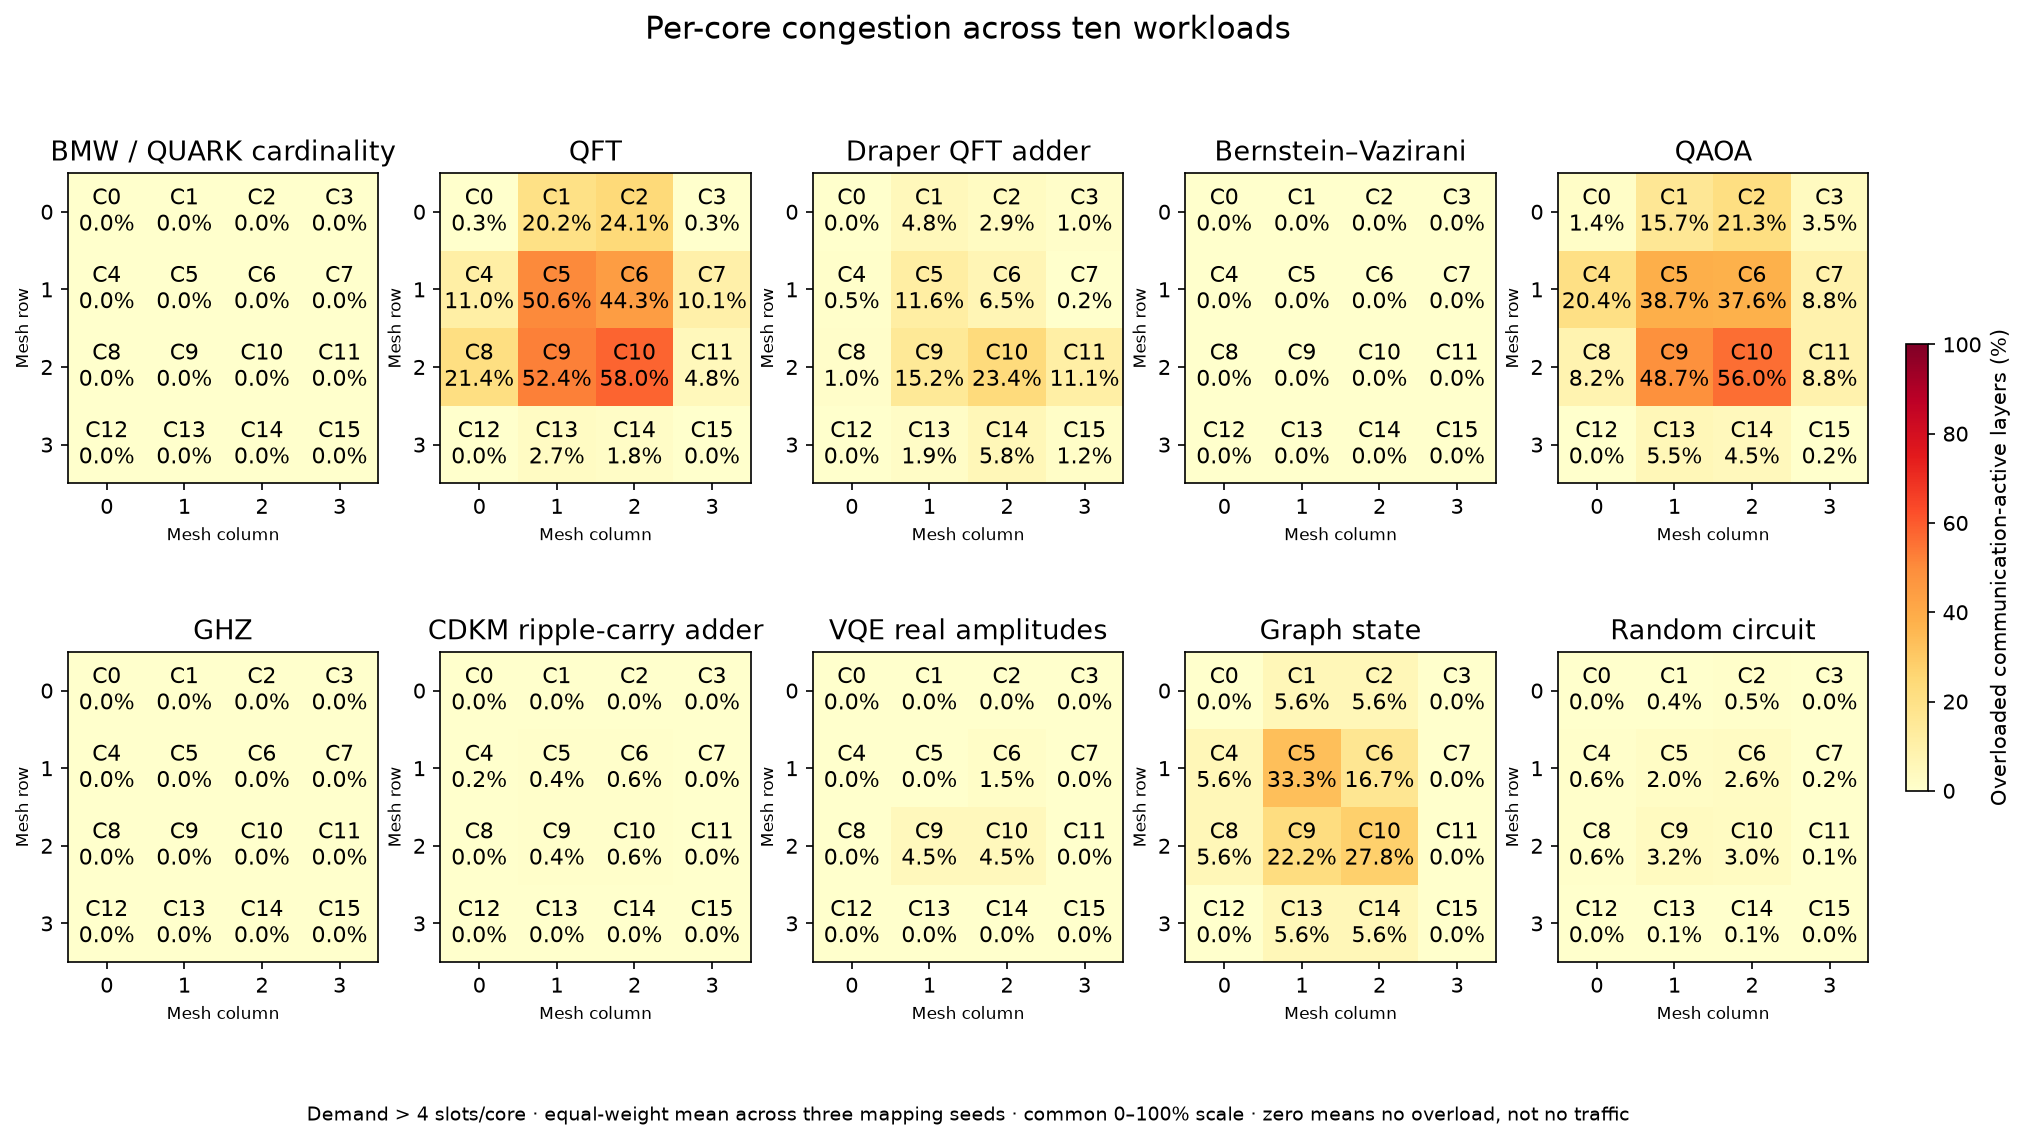
\includegraphics[width=\linewidth,height=0.80\textheight,keepaspectratio]{per_core_congestion.png}
\caption{Per-core congestion on the mesh: percentage of communication-active layers in which a core's demand exceeds 4 slots (mean over three mapping seeds). All 160 cells match the project's earlier figure at 0.1\% resolution.}
\label{fig:heatmap}
\end{figure}
\end{landscape}

\begin{table}[H]
\centering\small
\begin{tabular}{@{}lrrr@{}}
\toprule
Workload & Active layers (seeds 42/43/44) & Layers with any overload & Hottest core \\
\midrule
GHZ & 15/15/15 & 0.0\% & C0 (0.0\%) \\
Bernstein--Vazirani & 16/16/16 & 0.0\% & C0 (0.0\%) \\
BMW/QUARK cardinality & 90/90/90 & 0.0\% & C0 (0.0\%) \\
VQE real amplitudes & 22/22/22 & 6.1\% & C9 (4.5\%) \\
CDKM ripple-carry adder & 157/157/157 & 0.6\% & C6 (0.6\%) \\
Graph state & 6/6/6 & 33.3\% & C5 (33.3\%) \\
Draper QFT adder & 138/138/138 & 41.3\% & C10 (23.4\%) \\
QAOA & 163/163/163 & 71.6\% & C10 (56.0\%) \\
QFT & 112/112/112 & 65.2\% & C10 (58.0\%) \\
Random circuit & 2296/2296/2296 & 8.0\% & C9 (3.2\%) \\
\bottomrule
\end{tabular}
\caption{Structural overload at capacity 4, pooled over the three mapping seeds.}
\label{tab:heatmap}
\end{table}


Congestion concentrates on the central cores, which lie on the most shortest paths. QFT and QAOA are the heavy cases, graph state is
overloaded in a third of its (few) active layers, and GHZ, Bernstein--Vazirani and BMW never exceed four.

\section{Own demand against relay demand (Experiment 2)}
A \emph{route} is a qubit's consecutive hops within one layer; its first source and final destination are its \emph{endpoints}, every core in
between is a \emph{relay}. For a core and a layer, $D$ counts the hops touching the core, $D_{\mathrm{end}}$ those where the core is an endpoint of the
route, and $D_{\mathrm{relay}}$ the rest, so that a relay (touched by an arriving and a leaving hop) contributes two: $D=D_{\mathrm{end}}+D_{\mathrm{relay}}$.
With capacity $C$, a layer is overloaded for the core when $D>C$. It is \emph{own-overloaded} when $D_{\mathrm{end}}>C$, and \emph{relay-only-overloaded}
when $D_{\mathrm{end}}\le C<D$. The two sets are disjoint and together are exactly the overloaded layers.

\paragraph{Validation.} Own plus relay-only reproduces all 160 heatmap cells, and the per-core relay incidences, incident hops and peak layer demand reproduce
all 480 per-trial rows of the archive's per-core file exactly.

\paragraph{Counting qubits in flight.} A second variant counts routes instead of hops: under per-qubit ordering the hops of a route run one after
another, so a relay needs one memory for the route at a time, not two.


\begin{table}[H]
\centering\small
\resizebox{\ifdim\width>\linewidth\linewidth\else\width\fi}{!}{%
\begin{tabular}{@{}lrrrr@{}}
\toprule
Workload & C=1 & C=2 & C=3 & C=4 \\
\midrule
GHZ & 0.0\% & none & none & none \\
Bernstein--Vazirani & 0.0\% & none & none & none \\
BMW/QUARK cardinality & 0.0\% & none & none & none \\
VQE real amplitudes & 2.0\% & 0.0\% & 0.0\% & 0.0\% \\
CDKM ripple-carry adder & 0.4\% & 0.0\% & 0.0\% & 0.0\% \\
Graph state & 26.0\% & 9.5\% & 0.0\% & 0.0\% \\
Draper QFT adder & 54.5\% & 6.9\% & 6.4\% & 0.0\% \\
QAOA & 51.9\% & 14.9\% & 2.3\% & 0.4\% \\
QFT & 76.8\% & 10.1\% & 7.1\% & 0.0\% \\
Random circuit & 15.7\% & 1.8\% & 0.0\% & 0.0\% \\
\bottomrule
\end{tabular}}
\caption{Share of overloaded core-layers caused by a core's own endpoint demand (hop counting); the rest is relay-only overload.}
\label{tab:exp2-hop}
\end{table}

\begin{table}[H]
\centering\small
\begin{tabular}{@{}lrrrr@{}}
\toprule
Workload & C=1 & C=2 & C=3 & C=4 \\
\midrule
GHZ & none & none & none & none \\
Bernstein--Vazirani & none & none & none & none \\
BMW/QUARK cardinality & none & none & none & none \\
VQE real amplitudes & 5.3\% & 0.0\% & none & none \\
CDKM ripple-carry adder & 10.7\% & 0.0\% & 0.0\% & 0.0\% \\
Graph state & 37.5\% & 18.2\% & 0.0\% & 0.0\% \\
Draper QFT adder & 76.0\% & 9.5\% & 17.1\% & 0.0\% \\
QAOA & 59.7\% & 20.7\% & 4.5\% & 1.2\% \\
QFT & 86.8\% & 11.5\% & 12.8\% & 0.0\% \\
Random circuit & 39.6\% & 7.0\% & 0.0\% & 0.0\% \\
\bottomrule
\end{tabular}
\caption{Share of overloaded core-layers caused by a core's own endpoint demand (route counting); the rest is relay-only overload.}
\label{tab:exp2-route}
\end{table}


\begin{table}[H]
\centering\small
\resizebox{\ifdim\width>\linewidth\linewidth\else\width\fi}{!}{%
\begin{tabular}{@{}llrrrrr@{}}
\toprule
Workload & Hottest core & Overloaded \% & Own \% & Relay-only \% & Relay share of demand & Relay share of excess \\
\midrule
GHZ & none & 0.0 & 0.0 & 0.0 & -- & -- \\
Bernstein--Vazirani & none & 0.0 & 0.0 & 0.0 & -- & -- \\
BMW/QUARK cardinality & none & 0.0 & 0.0 & 0.0 & -- & -- \\
VQE real amplitudes & C9 & 4.5 & 0.0 & 4.5 & 80\% & 100\% \\
CDKM ripple-carry adder & C6 & 0.6 & 0.0 & 0.6 & 85\% & 100\% \\
Graph state & C5 & 33.3 & 0.0 & 33.3 & 93\% & 100\% \\
Draper QFT adder & C10 & 23.4 & 0.0 & 23.4 & 81\% & 100\% \\
QAOA & C10 & 56.0 & 0.0 & 56.0 & 81\% & 100\% \\
QFT & C10 & 58.0 & 0.0 & 58.0 & 78\% & 100\% \\
Random circuit & C9 & 3.2 & 0.0 & 3.2 & 87\% & 100\% \\
\bottomrule
\end{tabular}}
\caption{Hottest core of each workload at capacity 4 (hop counting): percentage of active layers overloaded, split into own and relay-only, and the relay share of its demand and of its excess.}
\label{tab:exp2-hottest}
\end{table}

\begin{table}[H]
\centering\small
\resizebox{\ifdim\width>\linewidth\linewidth\else\width\fi}{!}{%
\begin{tabular}{@{}lrrr@{}}
\toprule
Workload & Peak demand $D$ & Peak endpoint demand $D_{\mathrm{end}}$ & Peak routes through one core \\
\midrule
GHZ & 2 & 1 & 1 \\
Bernstein--Vazirani & 2 & 1 & 1 \\
BMW/QUARK cardinality & 2 & 1 & 1 \\
VQE real amplitudes & 5 & 2 & 3 \\
CDKM ripple-carry adder & 9 & 2 & 5 \\
Graph state & 13 & 3 & 7 \\
Draper QFT adder & 11 & 4 & 7 \\
QAOA & 18 & 5 & 10 \\
QFT & 24 & 4 & 13 \\
Random circuit & 12 & 3 & 6 \\
\bottomrule
\end{tabular}}
\caption{Peak demand at one core in one layer, over all mapping seeds: how close endpoint demand comes to the capacity.}
\label{tab:exp2-peaks}
\end{table}


\paragraph{Why the counting matters.} Hop counting charges a relay two touches (one arriving hop, one leaving hop), but under per-qubit ordering those two hops run one after the other, so a relay needs one memory at a time. Hop counting therefore overstates
contention, most visibly at one slot: GHZ is structurally ``overloaded'' at one slot by hop counting (20\% of its layers) yet never waits in the simulator, and route counting, whose peak for GHZ is one route per core, correctly shows no contention. This is why Experiment~1 relates the
simulated cost to the structure and why both counts are reported.

\paragraph{Findings.} At the modelled capacity of four, almost all overload is relay overload. The peak endpoint demand is 4 for QFT and Draper, 5 for QAOA and at most 3
for the others, against a total demand up to 24. The only own-overload at capacity 4 is in QAOA, at the corner cores C0 and C3 (0.61\% of active layers each), which is
0.44\% of QAOA's overload. Smaller budgets bring own demand in: QFT is 77\% own-overload at capacity 1. A routing change can therefore remove at most the relay part;
the own part is a floor set by the mapping. Route counting finds less overload than hop counting (core C10 of QFT is overloaded in 46.4\% of active layers against
58.0\%) and relay traffic is still essentially all of what remains.

\section{Every capacity, both countings}
Capacity four is the modelled value; the smaller capacities show how the split moves as memory is removed. Each of the following landscape pages shows one capacity and counting with every workload that has overload side by side: for each workload the left heatmap is the percentage of active layers in which the core is overloaded by its own endpoint demand and the right heatmap the percentage in which it is overloaded only because of relay traffic. Per-core numbers for capacities four and two are in Appendix~\ref{app:percore}; the data for all capacities and both countings are in \code{results/experiment2_own_vs_relay_2026-10-24/}.
\begin{landscape}
\begin{figure}[p]
\centering
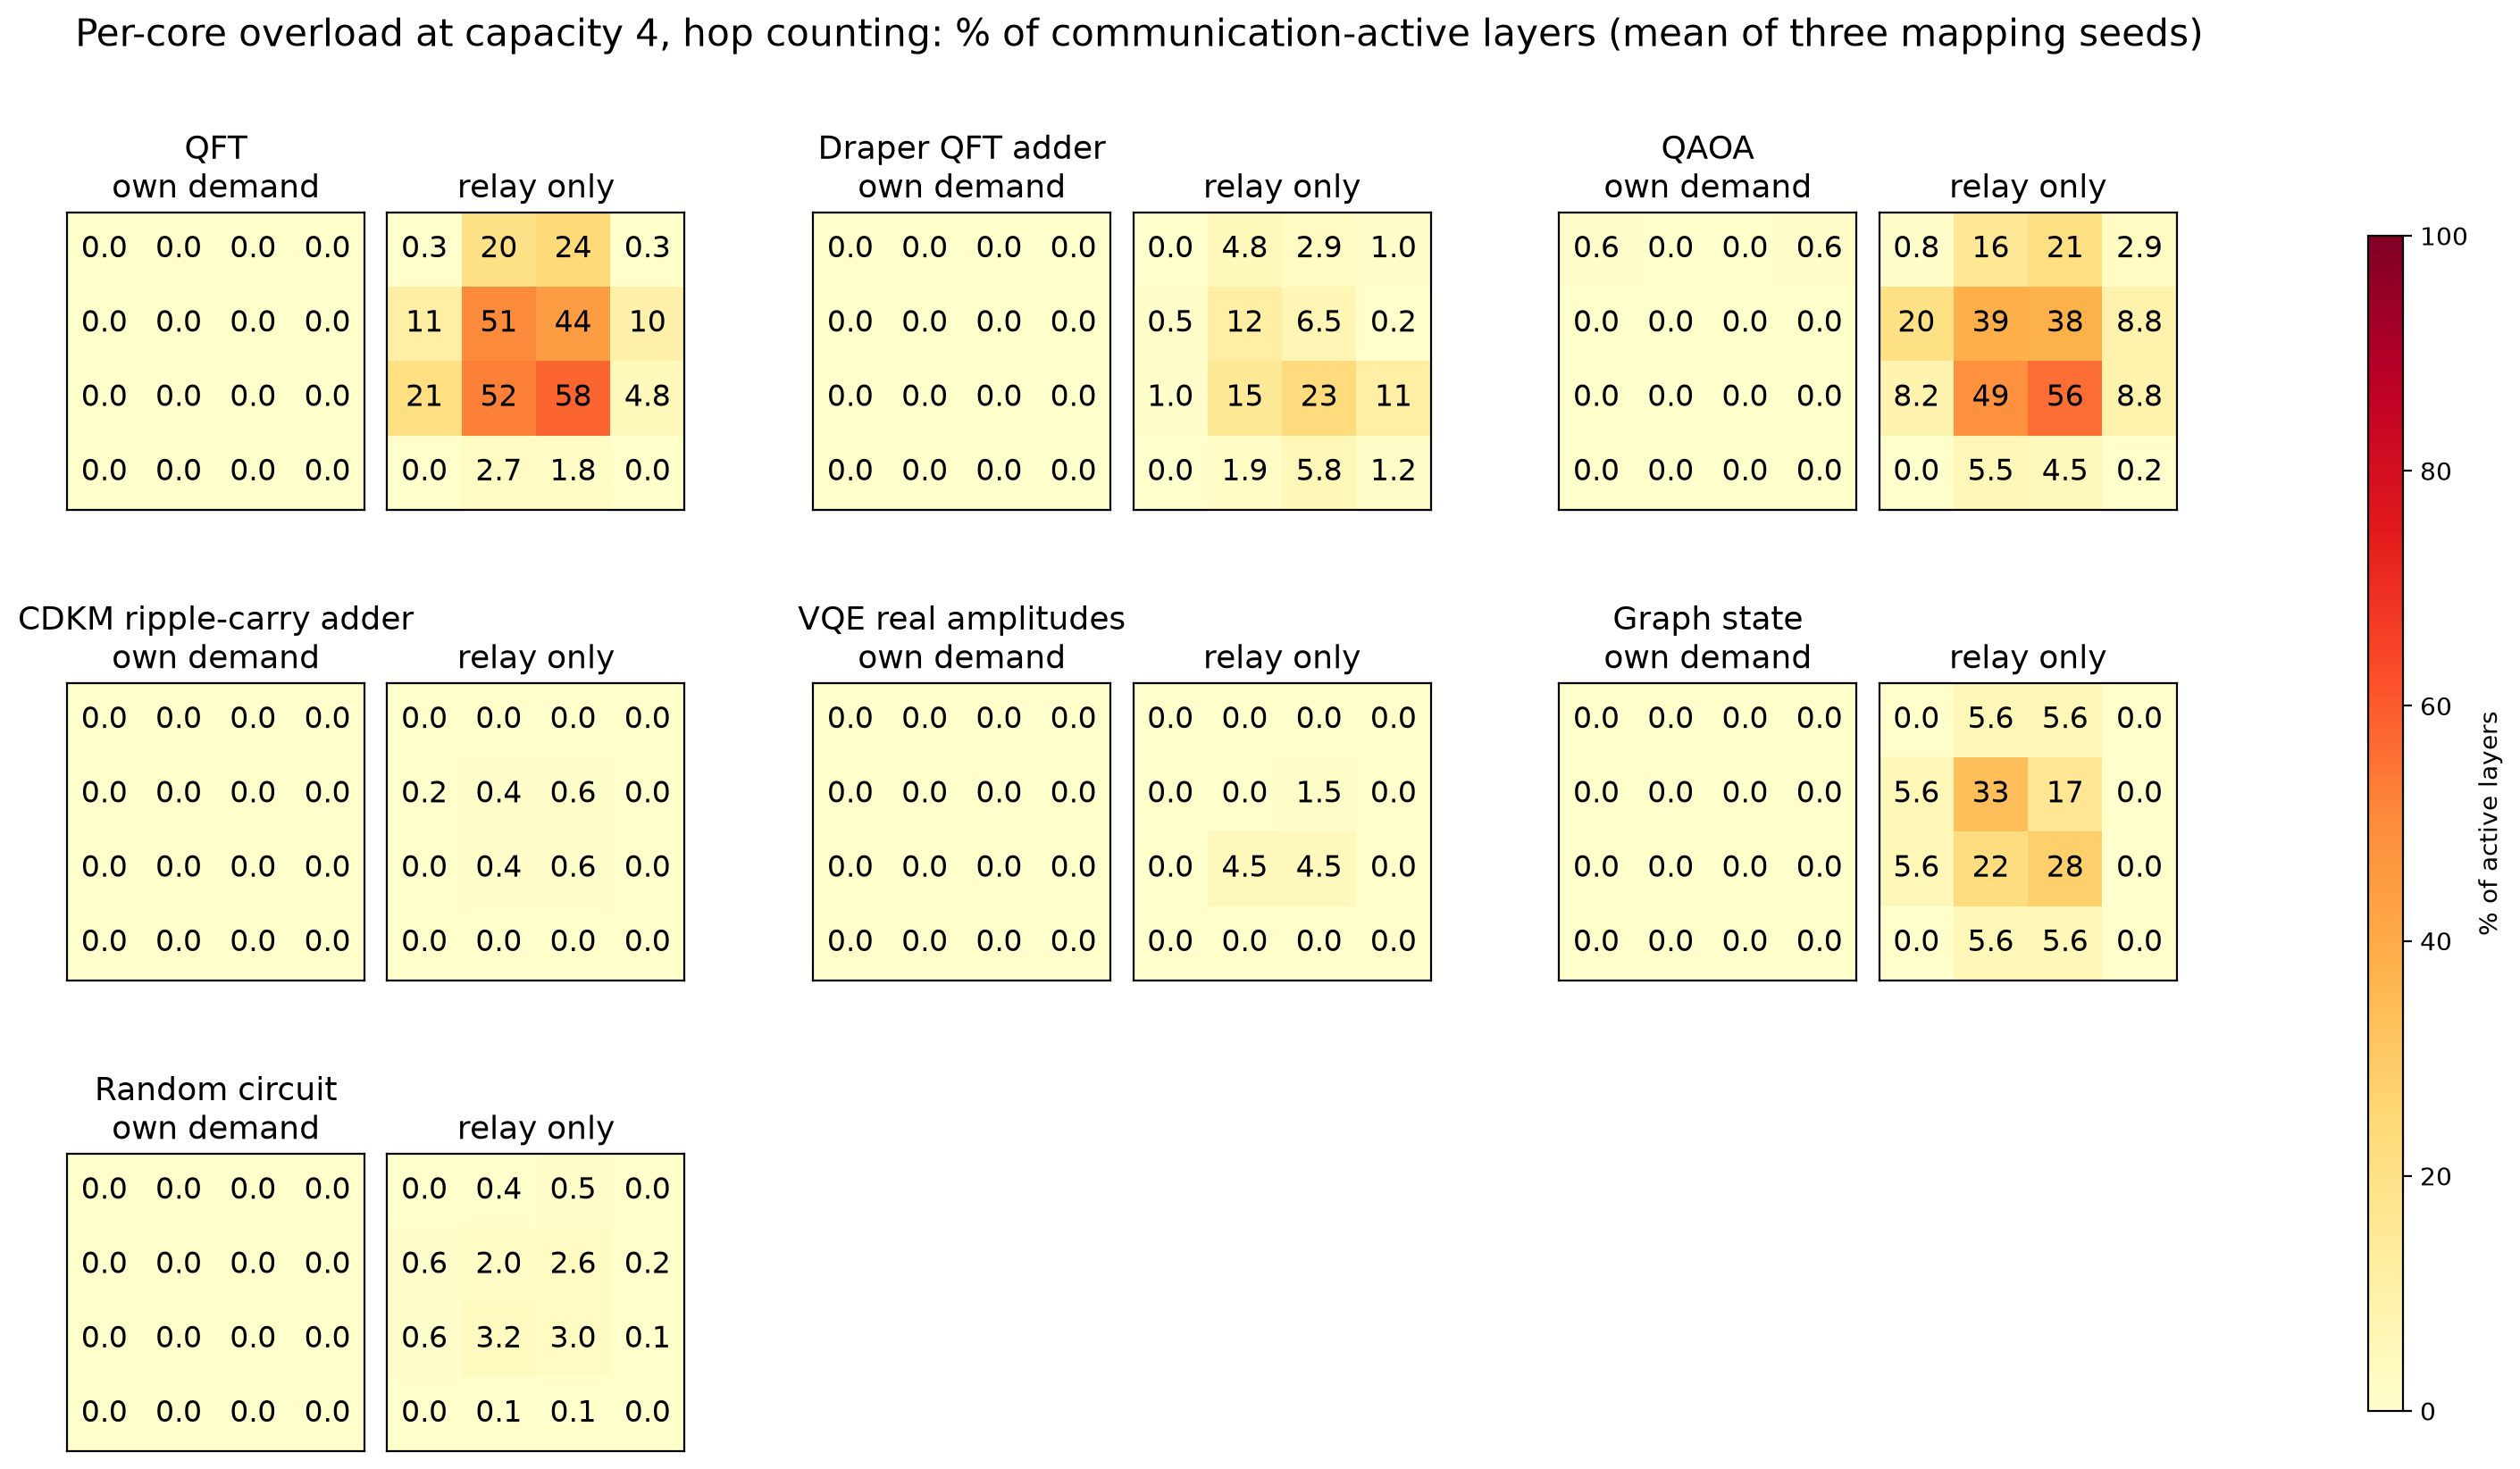
\includegraphics[width=\linewidth,height=0.80\textheight,keepaspectratio]{exp2_overview_c4_hop.png}
\caption{Capacity 4, hop counting. For each workload with overload, the left heatmap is the percentage of its active layers in which the core is overloaded by its own endpoint demand and the right heatmap the percentage in which it is overloaded only because of relay traffic. Mesh cores are numbered row by row (core 10 is row 2, column 2). Mean of three mapping seeds.}
\label{fig:exp2-overview-c4-hop}
\end{figure}
\end{landscape}
\begin{landscape}
\begin{figure}[p]
\centering
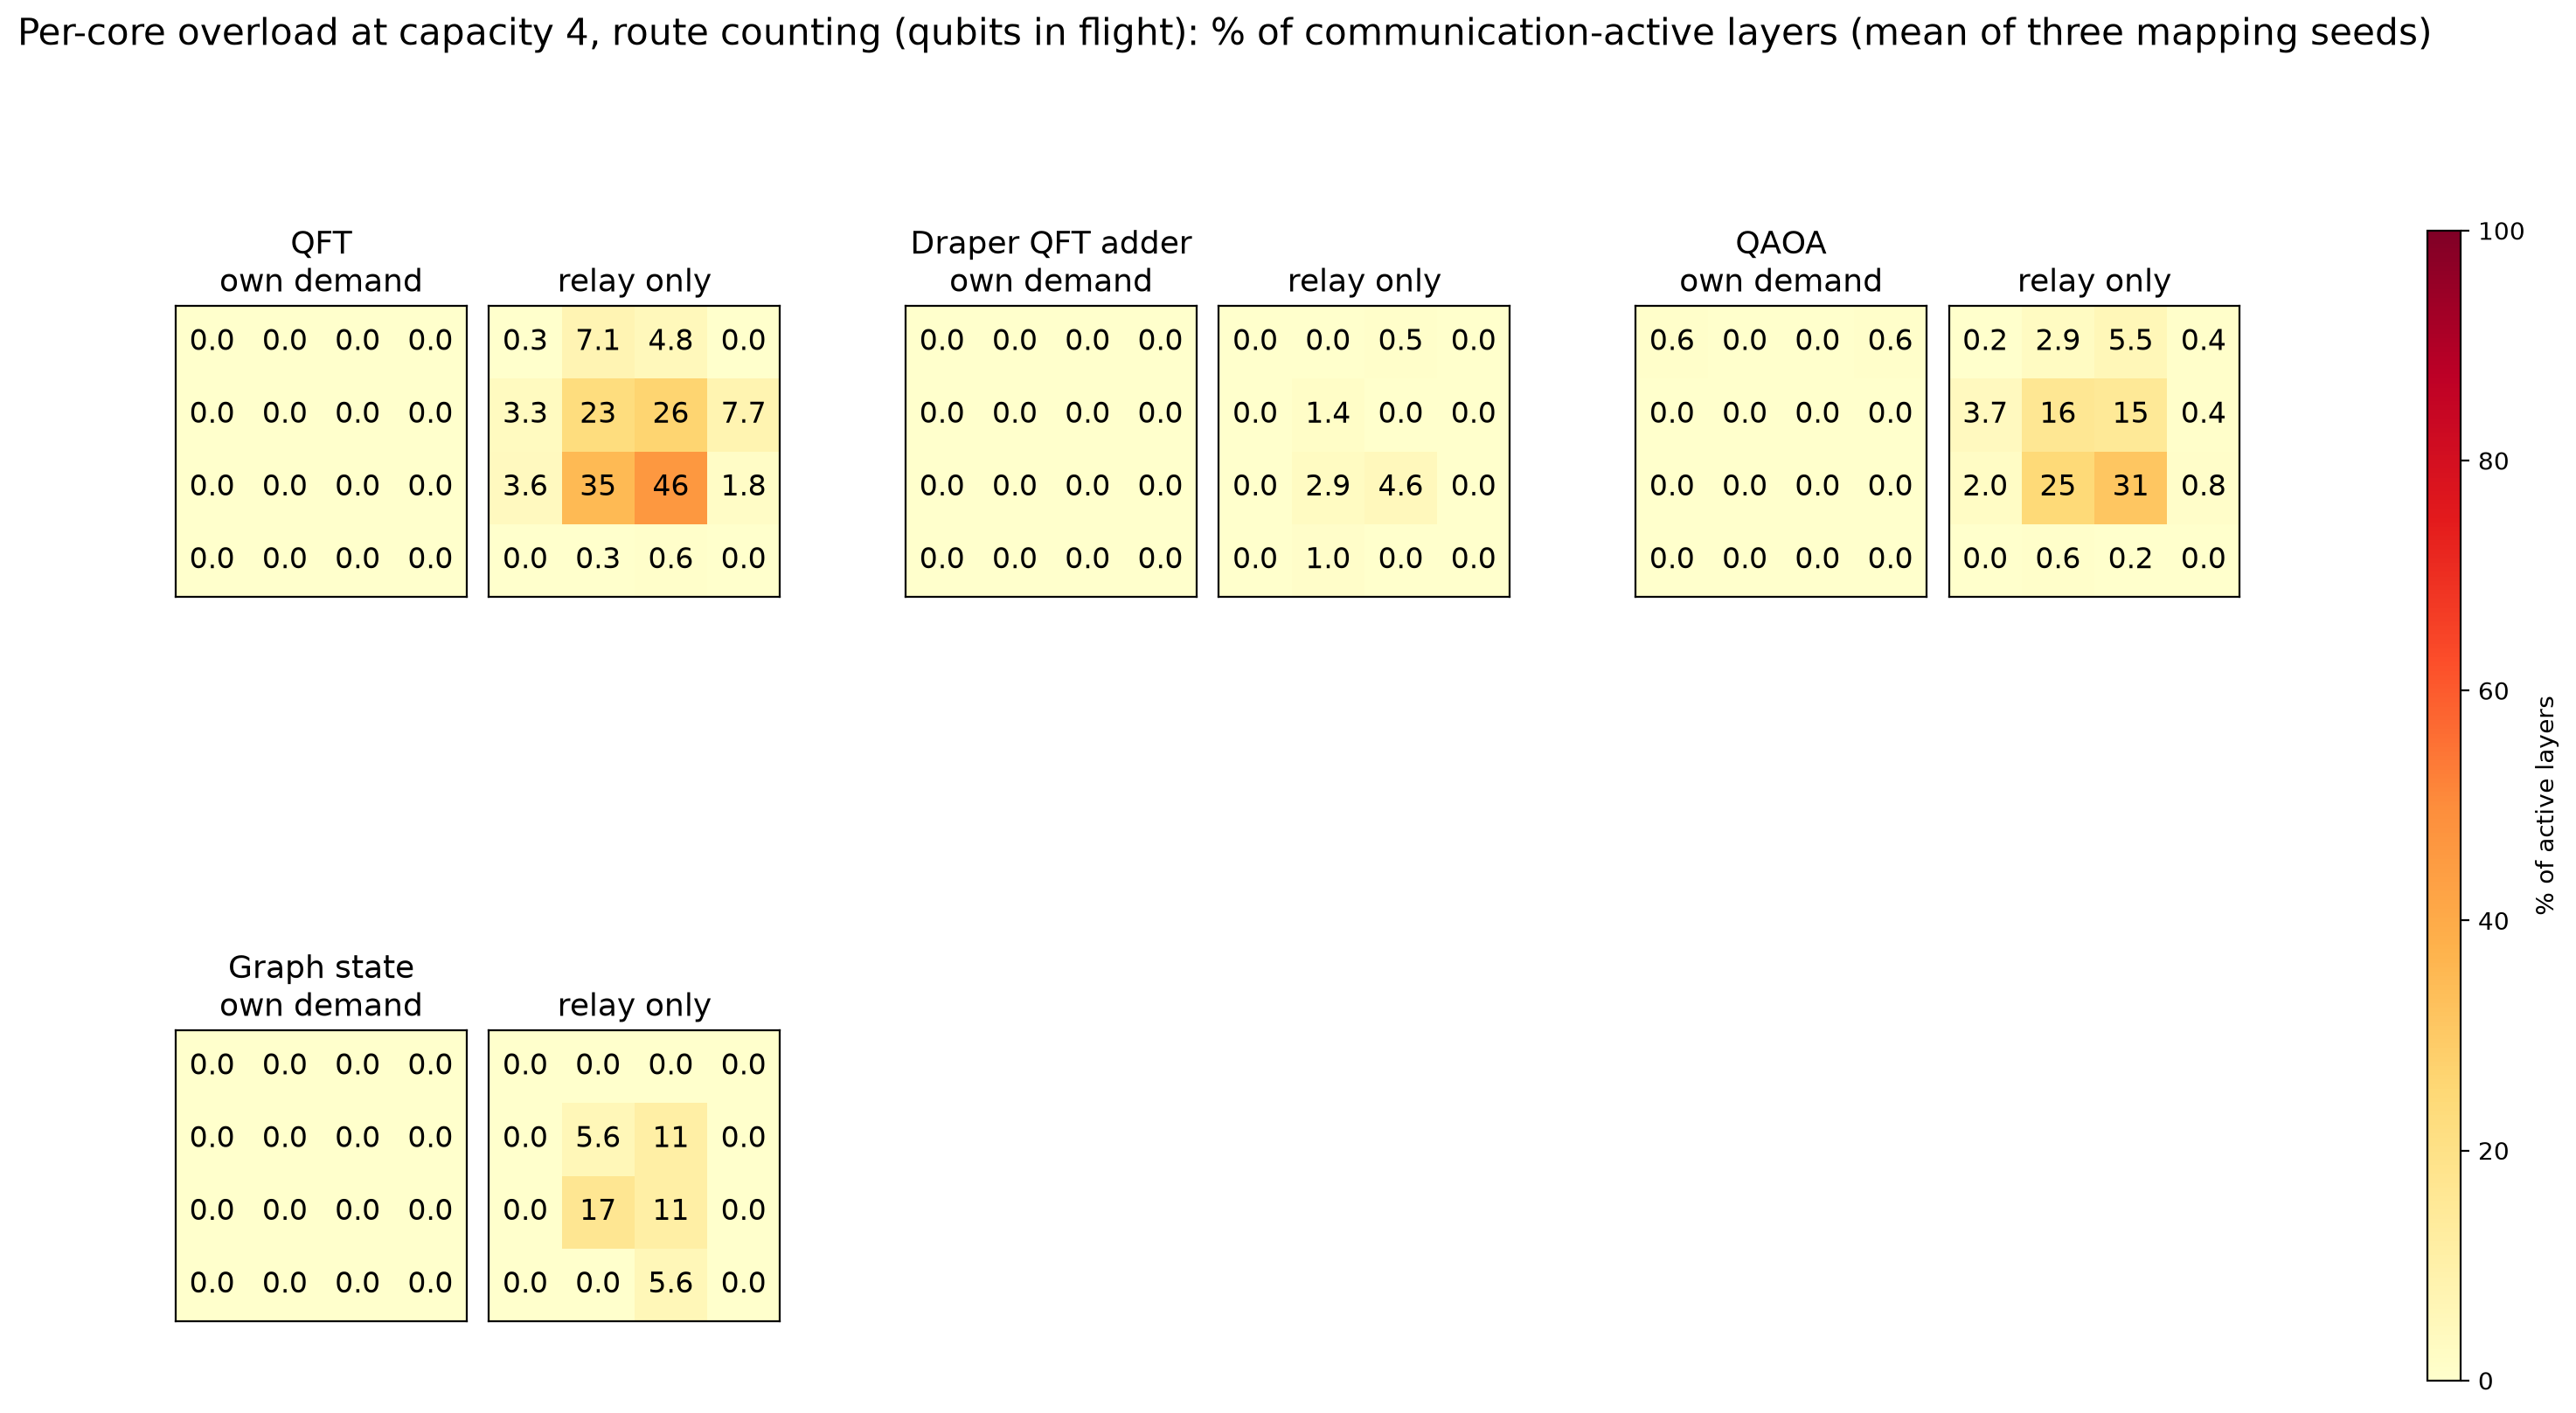
\includegraphics[width=\linewidth,height=0.80\textheight,keepaspectratio]{exp2_overview_c4_route.png}
\caption{Capacity 4, route counting (qubits in flight). For each workload with overload, the left heatmap is the percentage of its active layers in which the core is overloaded by its own endpoint demand and the right heatmap the percentage in which it is overloaded only because of relay traffic. Mesh cores are numbered row by row (core 10 is row 2, column 2). Mean of three mapping seeds.}
\label{fig:exp2-overview-c4-route}
\end{figure}
\end{landscape}
\begin{landscape}
\begin{figure}[p]
\centering
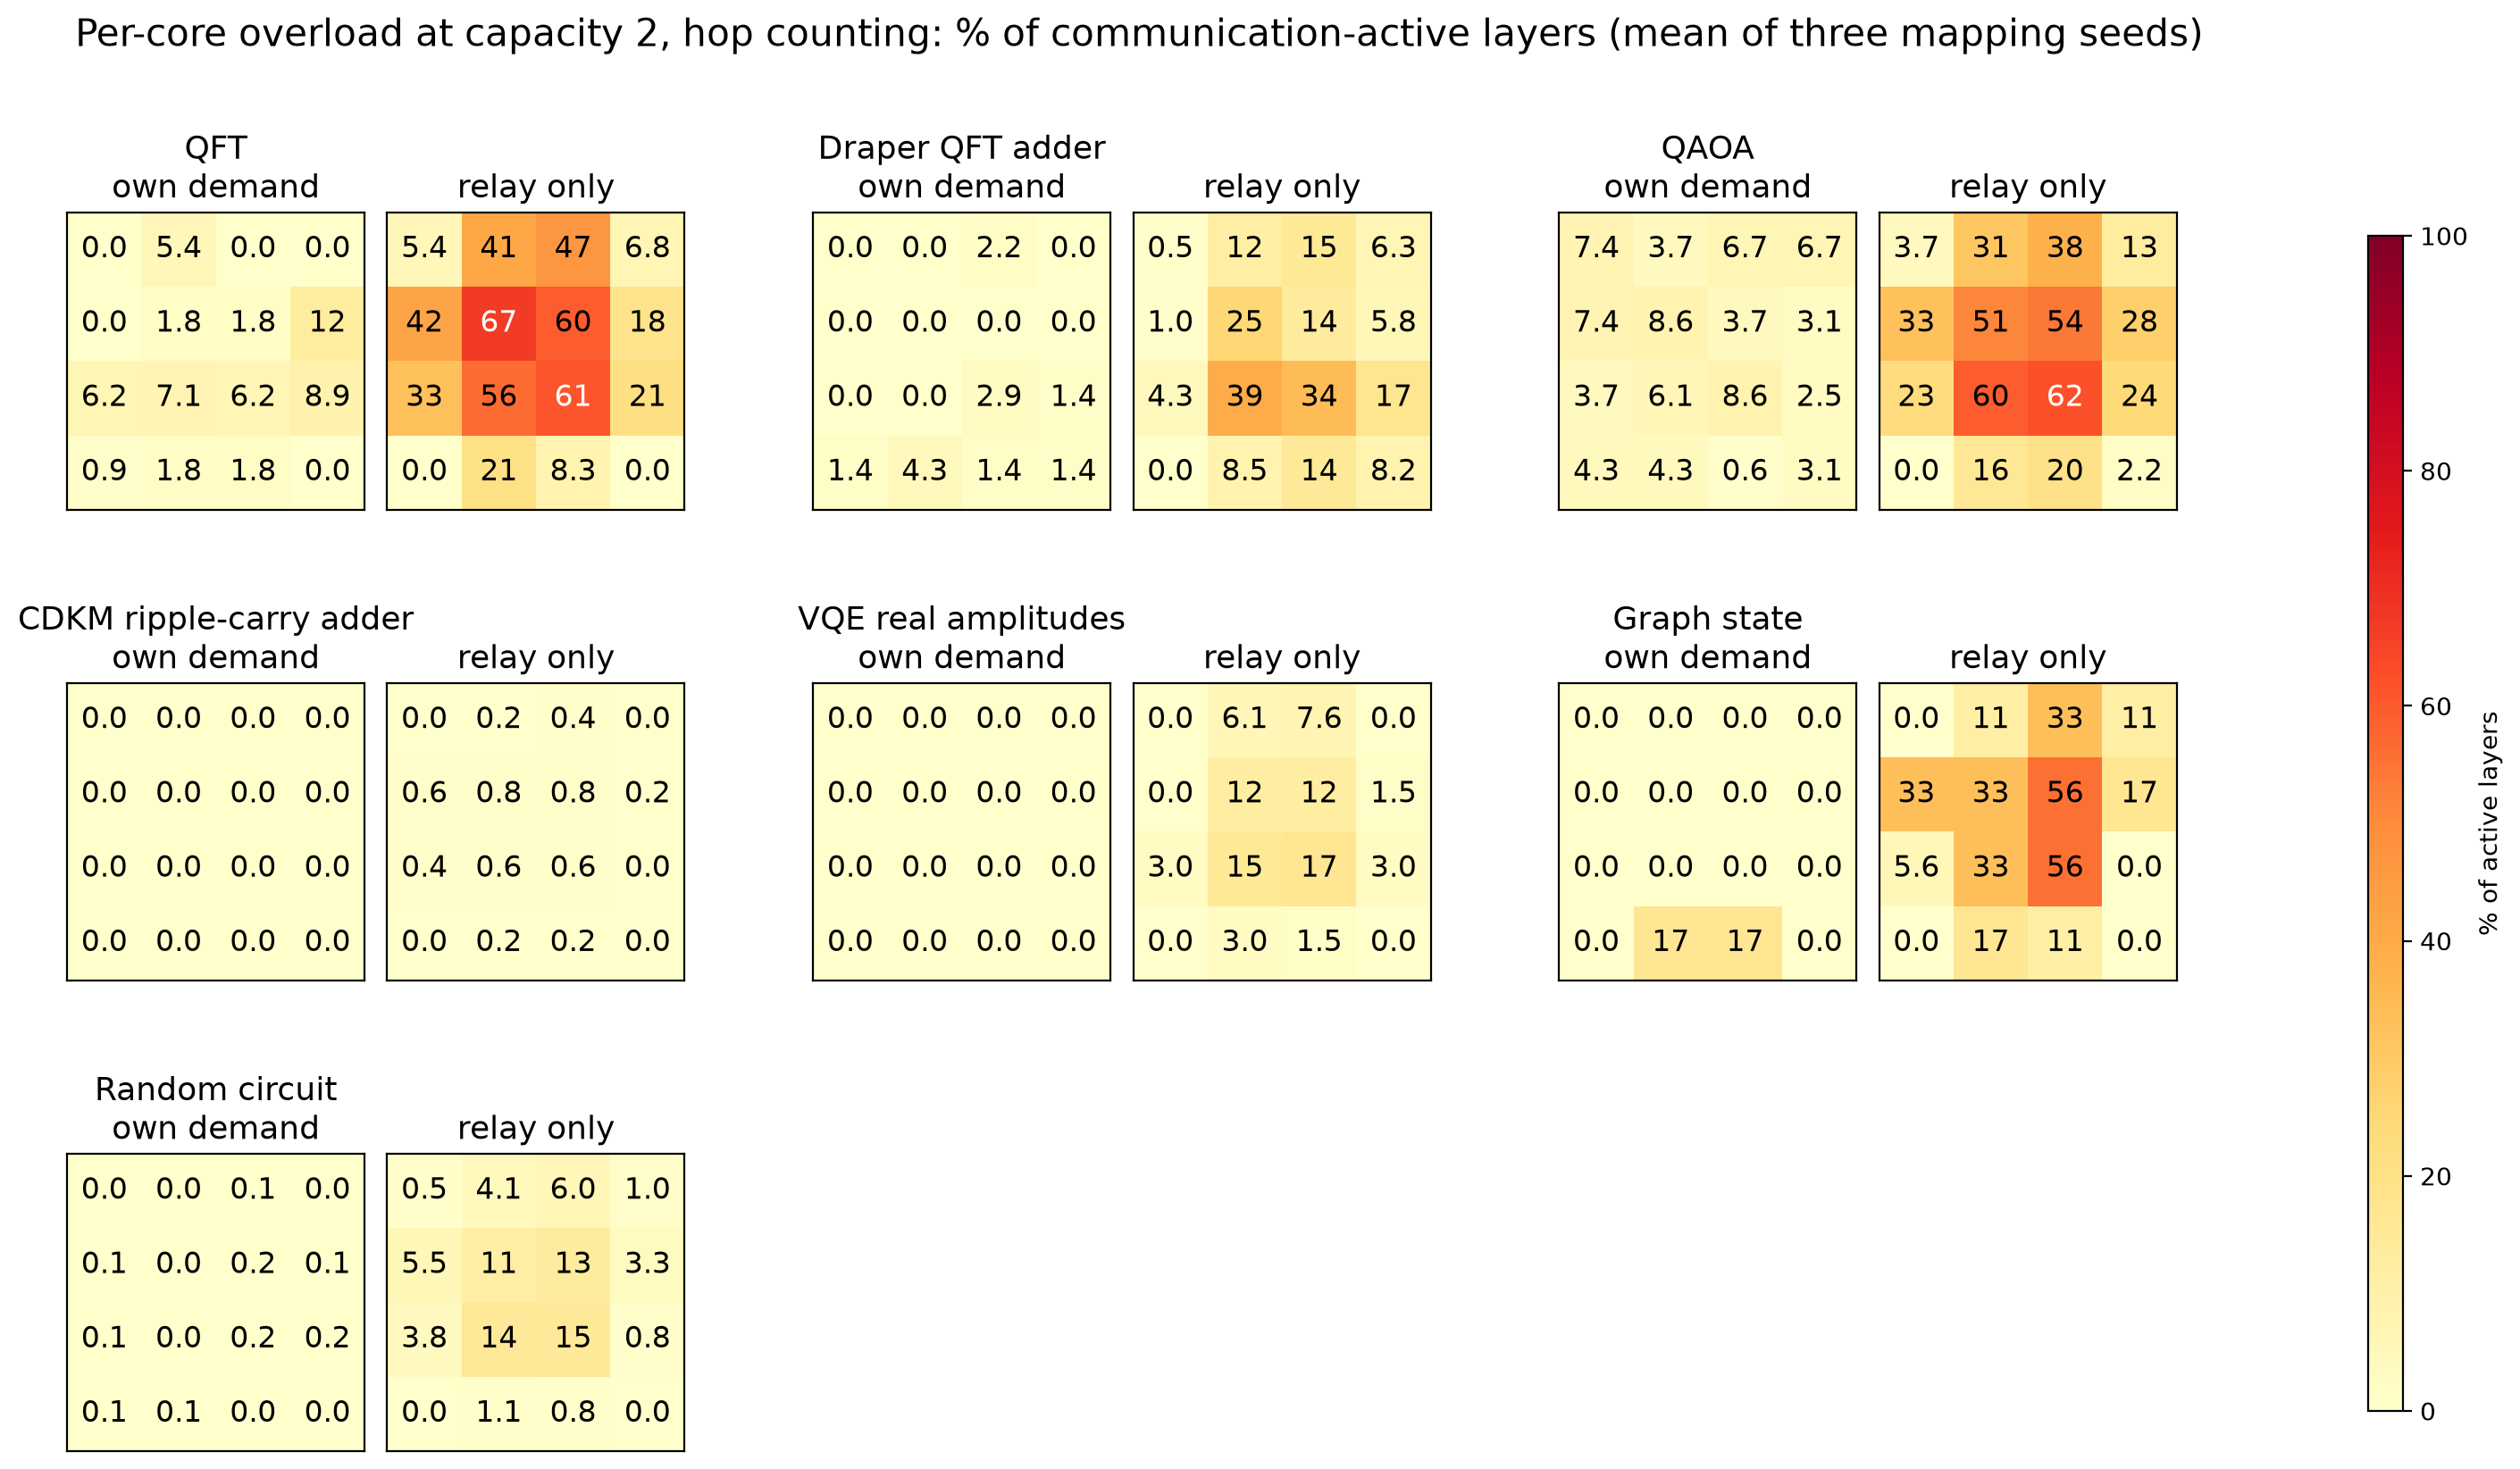
\includegraphics[width=\linewidth,height=0.80\textheight,keepaspectratio]{exp2_overview_c2_hop.png}
\caption{Capacity 2, hop counting. For each workload with overload, the left heatmap is the percentage of its active layers in which the core is overloaded by its own endpoint demand and the right heatmap the percentage in which it is overloaded only because of relay traffic. Mesh cores are numbered row by row (core 10 is row 2, column 2). Mean of three mapping seeds.}
\label{fig:exp2-overview-c2-hop}
\end{figure}
\end{landscape}
\begin{landscape}
\begin{figure}[p]
\centering
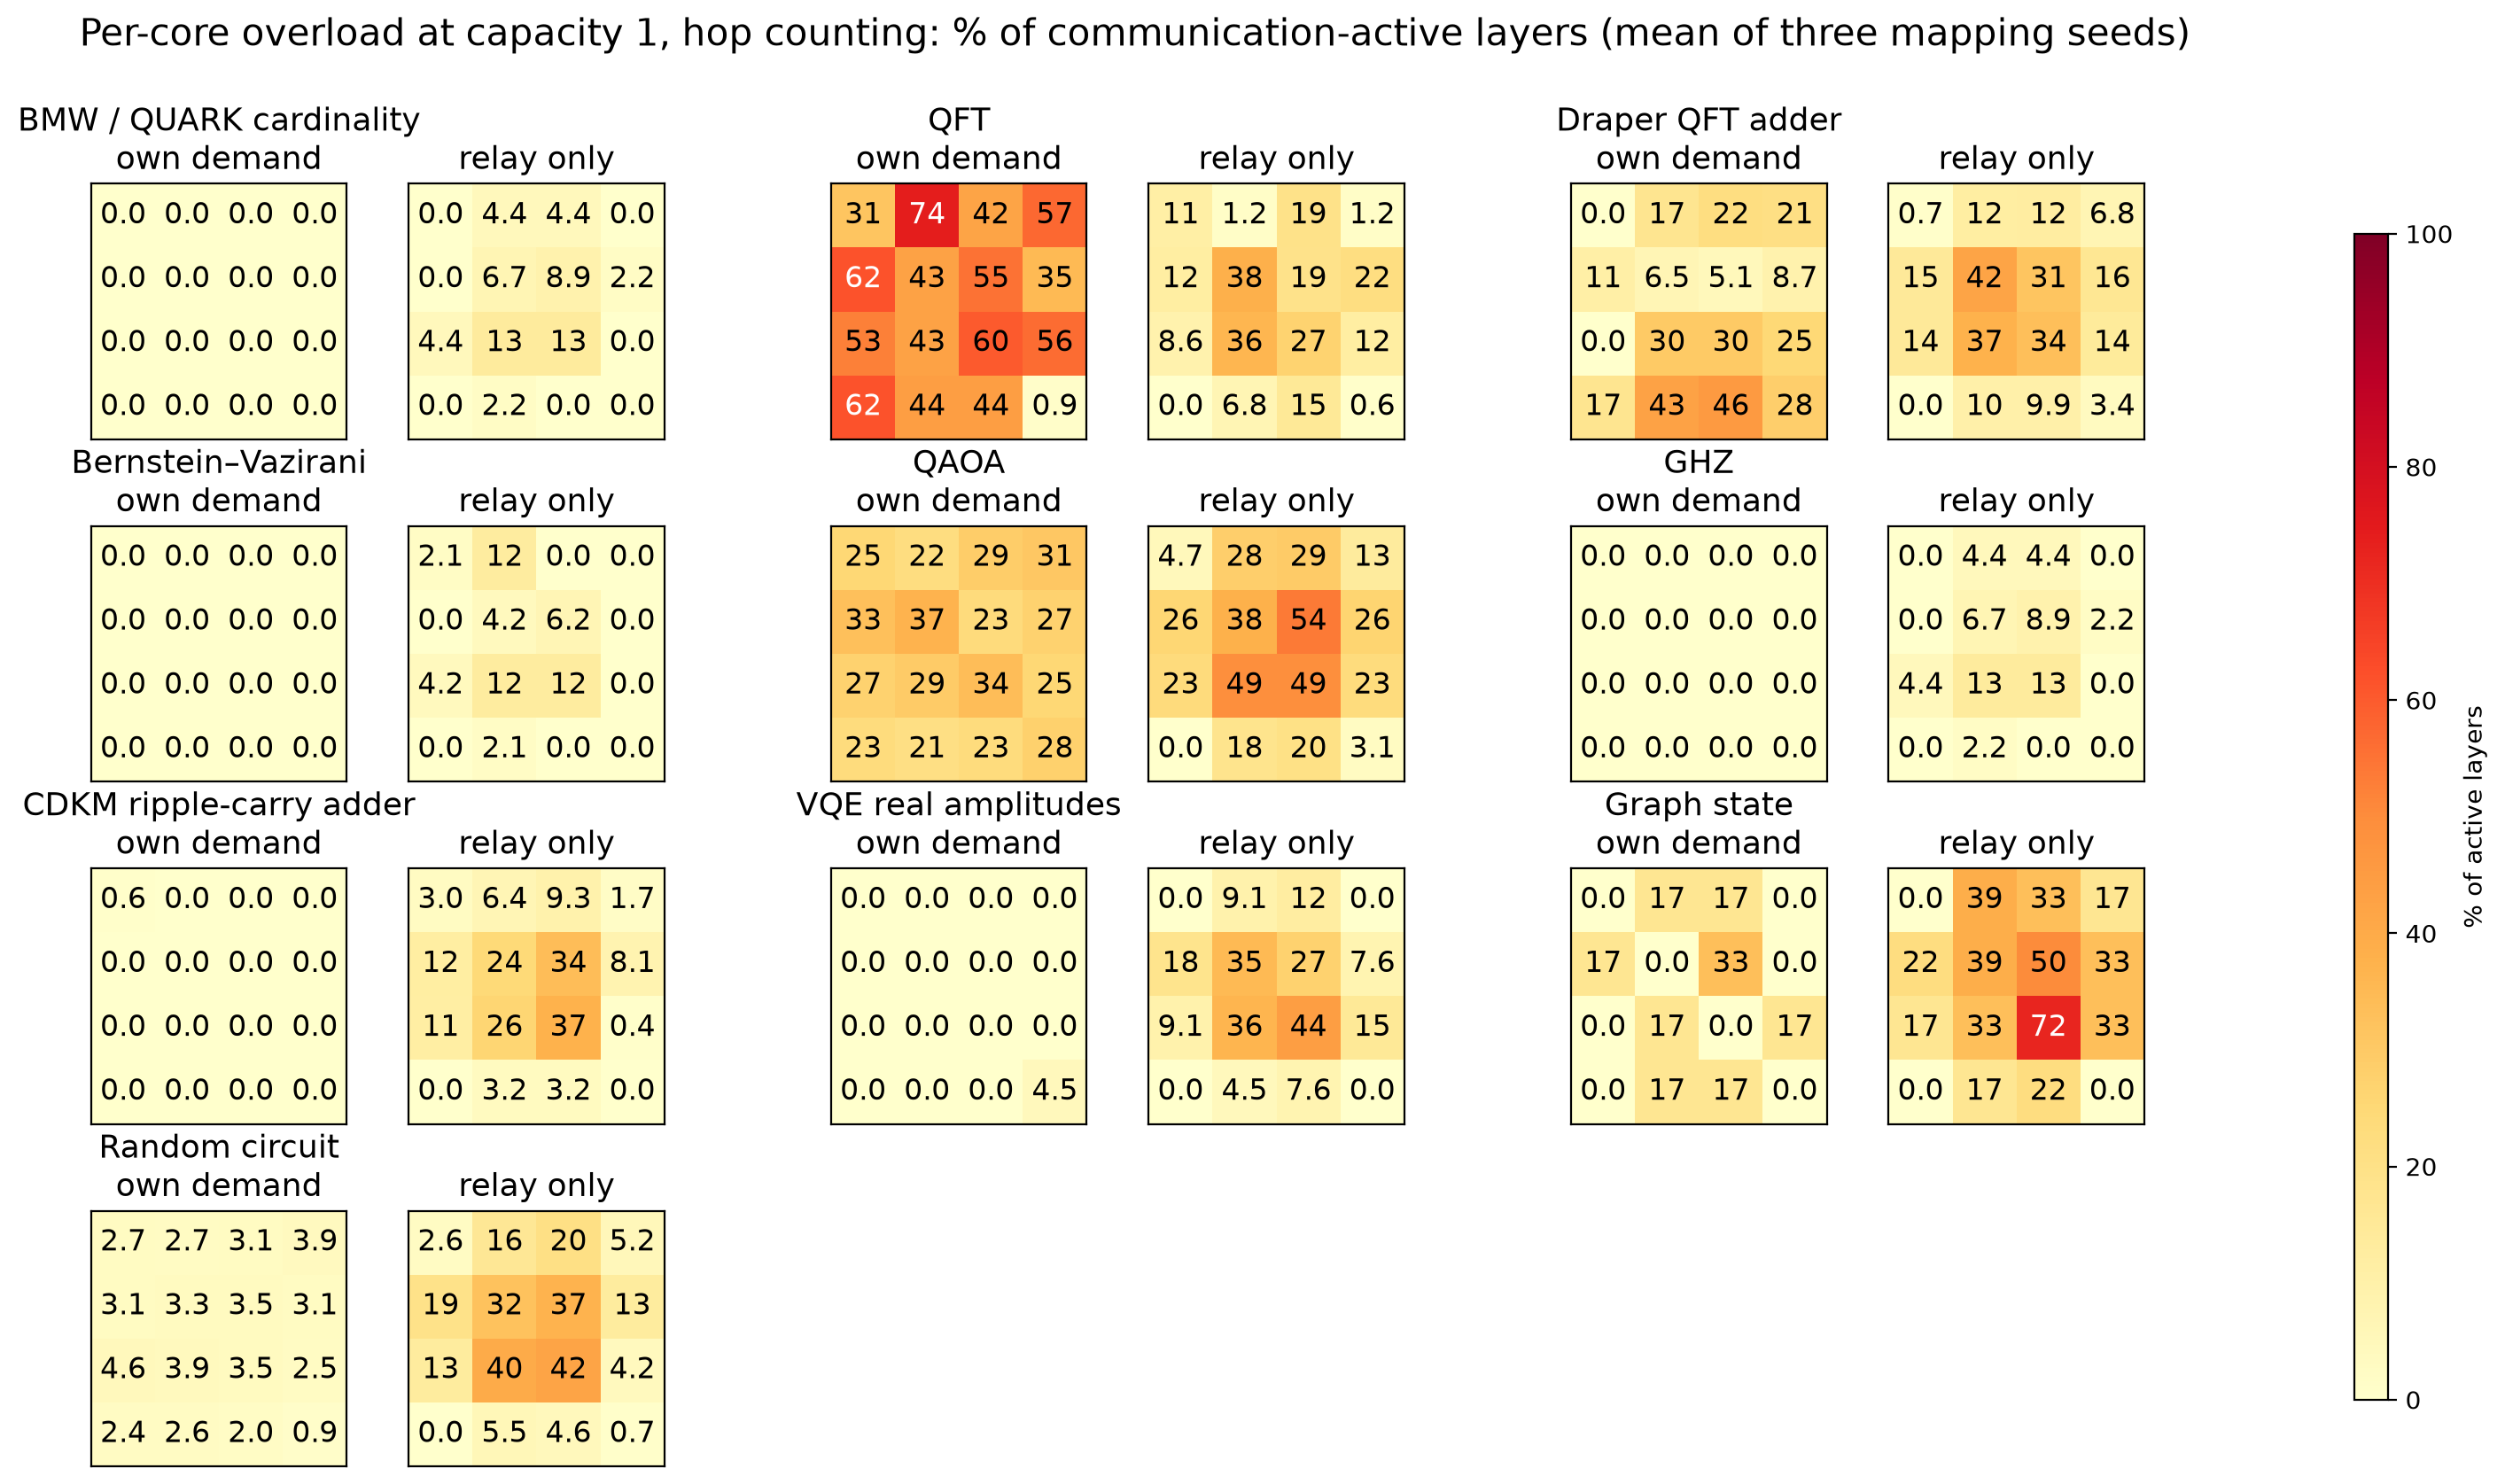
\includegraphics[width=\linewidth,height=0.80\textheight,keepaspectratio]{exp2_overview_c1_hop.png}
\caption{Capacity 1, hop counting. For each workload with overload, the left heatmap is the percentage of its active layers in which the core is overloaded by its own endpoint demand and the right heatmap the percentage in which it is overloaded only because of relay traffic. Mesh cores are numbered row by row (core 10 is row 2, column 2). Mean of three mapping seeds.}
\label{fig:exp2-overview-c1-hop}
\end{figure}
\end{landscape}
\begin{landscape}
\begin{figure}[p]
\centering
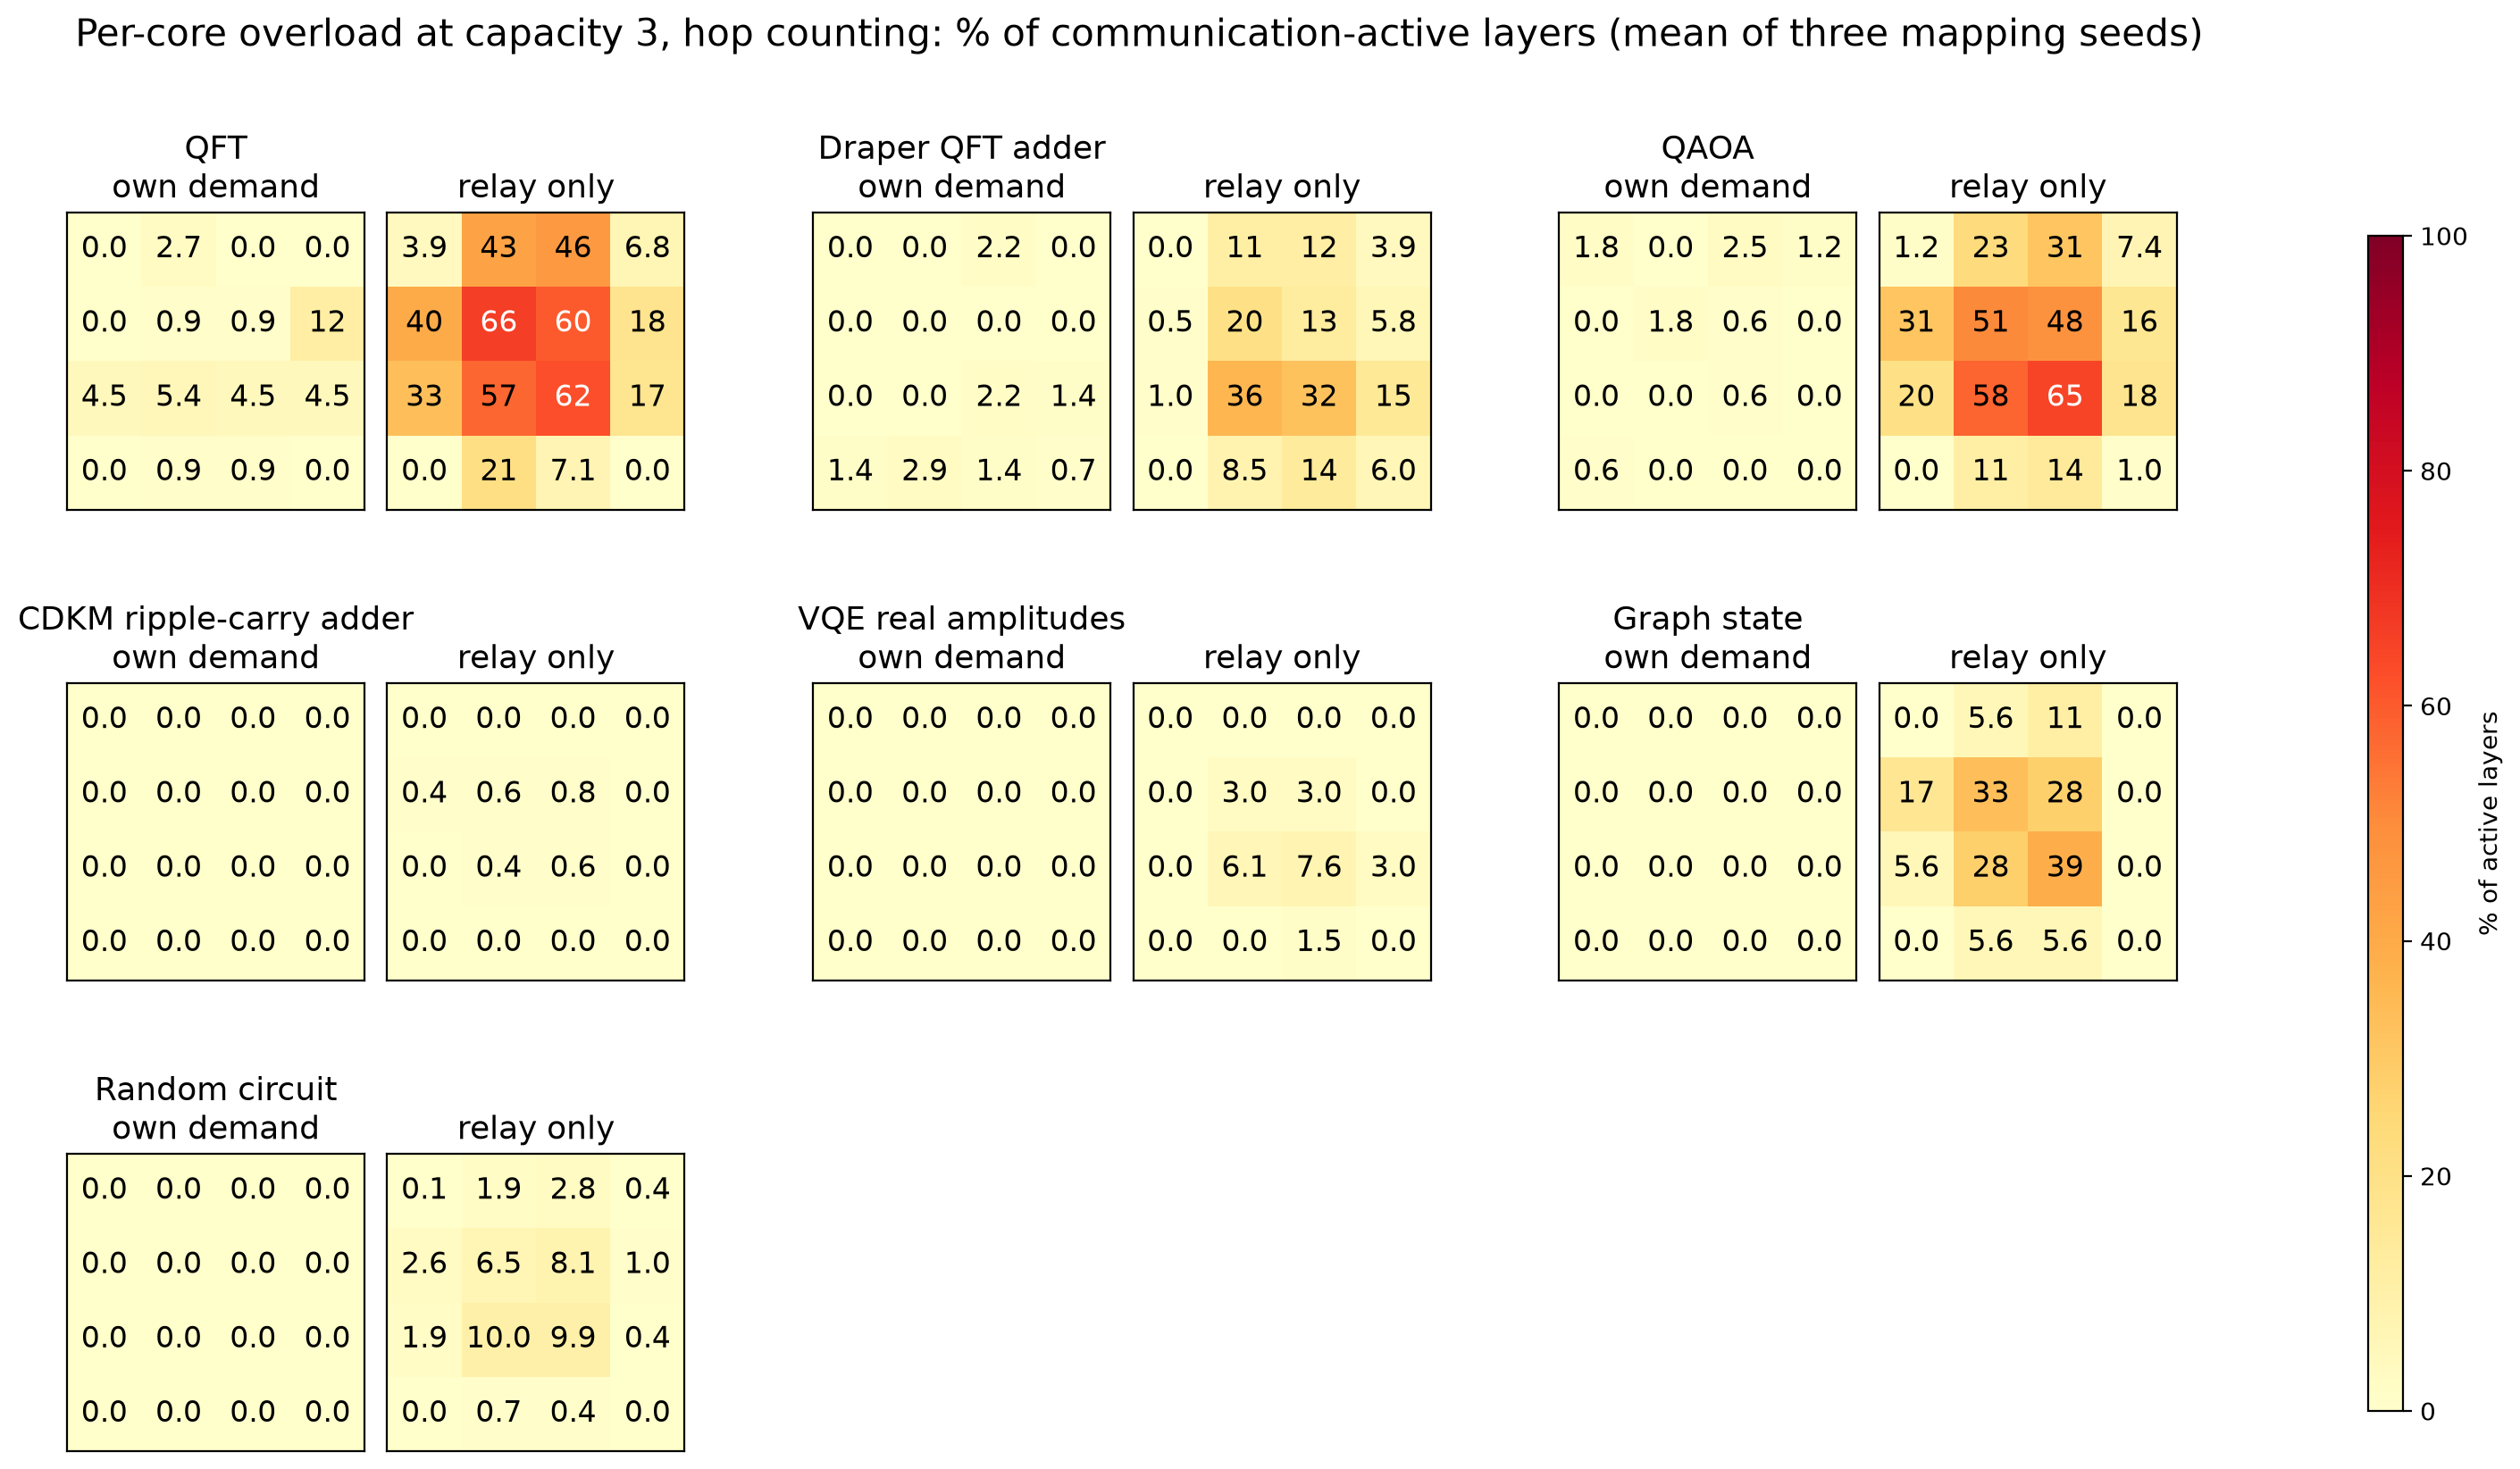
\includegraphics[width=\linewidth,height=0.80\textheight,keepaspectratio]{exp2_overview_c3_hop.png}
\caption{Capacity 3, hop counting. For each workload with overload, the left heatmap is the percentage of its active layers in which the core is overloaded by its own endpoint demand and the right heatmap the percentage in which it is overloaded only because of relay traffic. Mesh cores are numbered row by row (core 10 is row 2, column 2). Mean of three mapping seeds.}
\label{fig:exp2-overview-c3-hop}
\end{figure}
\end{landscape}

